\chapter{轮子}
\begin{figure}[htbp]
\centering
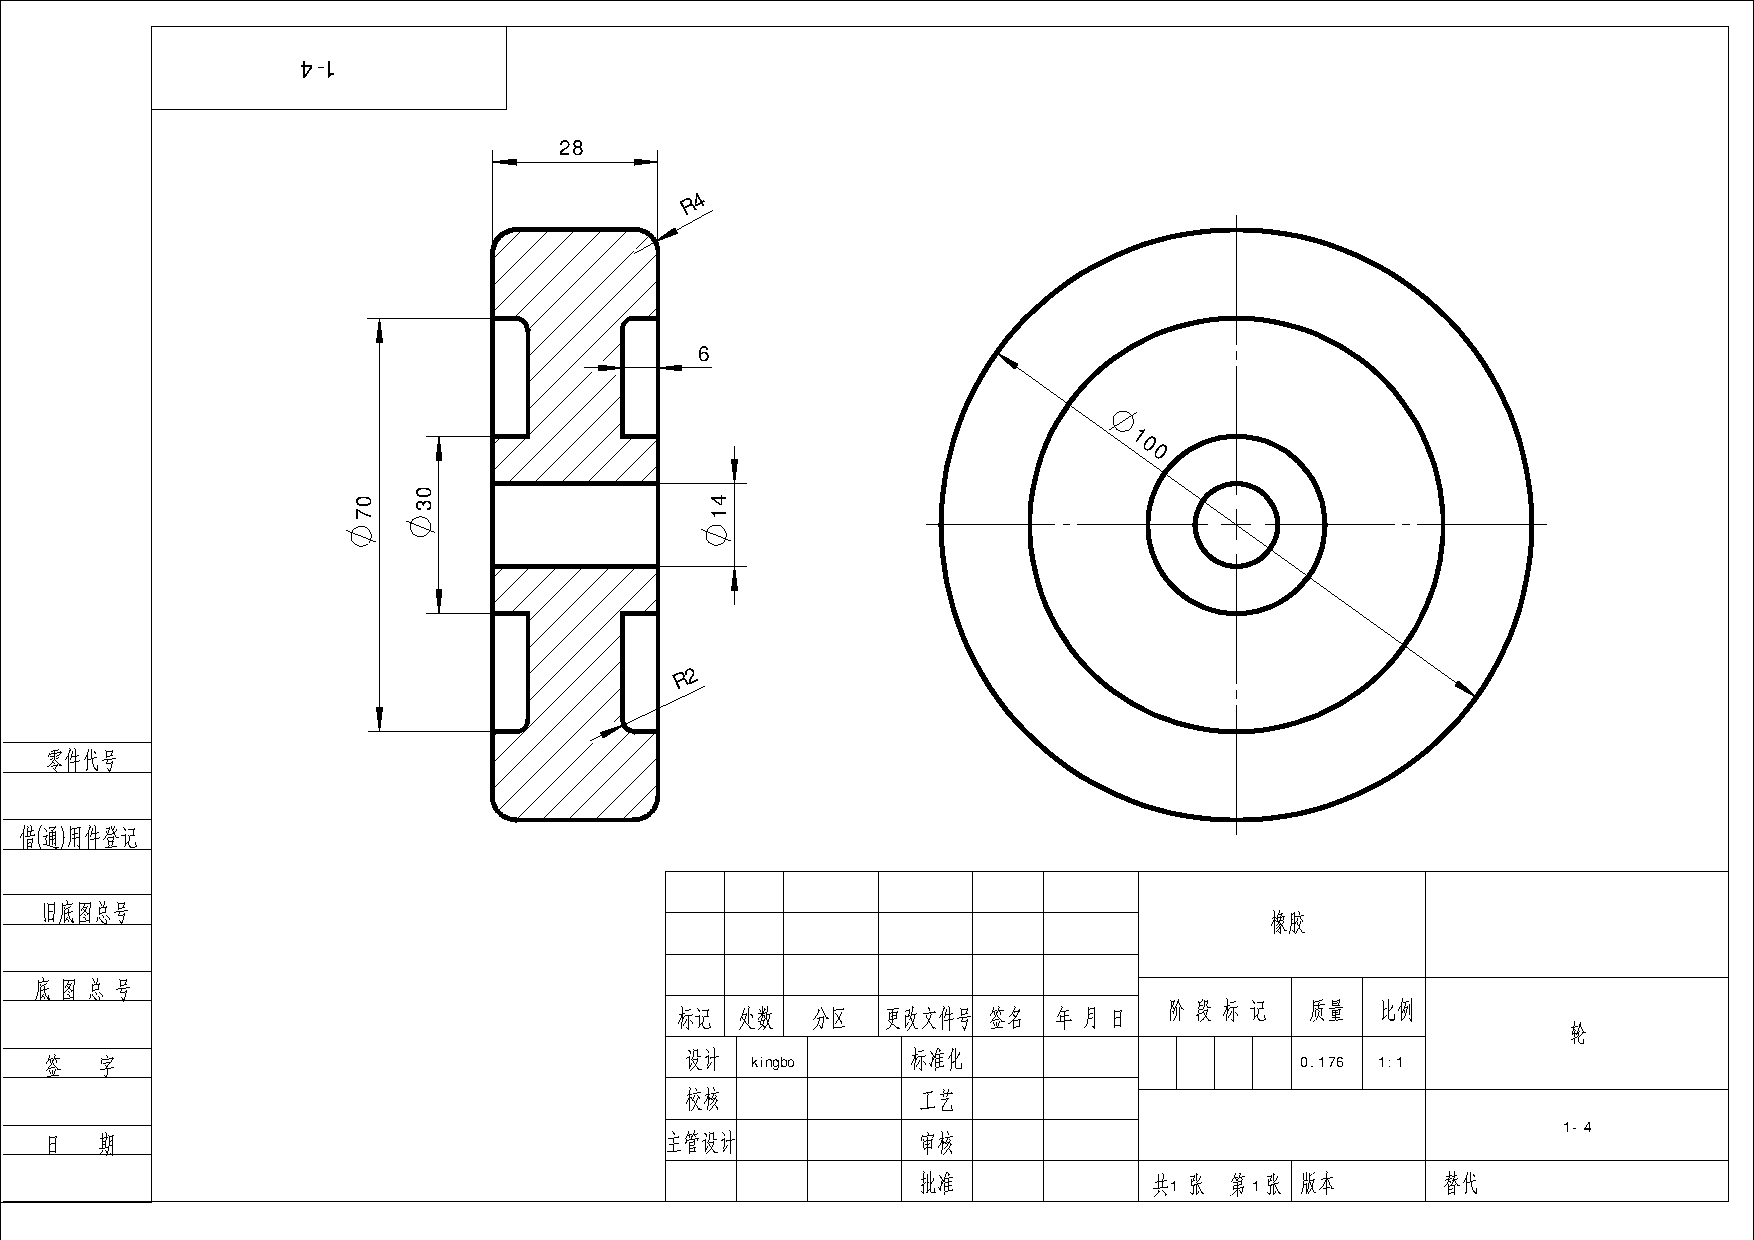
\includegraphics[scale=0.45]{xiaolunlun.pdf}
\caption{轮零件图}\label{fig:xiaolunlun.pdf}
\end{figure}

本章的目标是构建图\ref{fig:xiaolunlun.pdf}所示的小轮组轮零件的三维模型,并在此基础之上制作轮的零件图。因此本章重点讲解以下内容:
\begin{itemize}
\item 轮的三维模型构建
\item 剖视图的概念
\item 轮全剖视图的制作
\item 半径和直径尺寸的标注
\end{itemize}


%\section{标题栏、尺寸、文字}

\endinput
\endinput